\documentclass[a4paper,12pt]{extarticle}
\usepackage[russian]{babel}
\usepackage[utf8x]{inputenc}
\usepackage{indentfirst}
\usepackage{graphicx} 

\title{\textbf{Защита компьютерной информации}}
\author{Михальцов П.А.}

\begin{document}
	\maketitle
	\section{Защита информации в информационно вычислительных системах}
	\subsection{Проблемы защиты компьютерной информации}
	Вопросы 
	\begin{enumerate}
		\item Основное понятия об угрозах информационной безопасности
		\item Актуальность проблемы обеспечения информационной безопасности. Задачи защиты информации
		\item Задачи информационной безопасности
	\end{enumerate}
	\subsubsection{Основное понятия об угрозах информационной безопасности}
	\textbf{\textit{Информационная безопасность}} --- такое состояние системы, при которой она может противостоять против дестабилизирующий воздействию внешних и внутрений угроз, а также -- её функционирования не создаёт информационных угроз для элементов самой системы и внешней среды
	
	Обеспечение информационной безопасности проблемы может быть достигнуто лишь при взаимоувязанном решении трёх составляющих проблем:
	\begin{itemize}
		\item защита находящееся в системе информации от дестабилизирующего воздействия внешних и внутренних угроз информации
		\item защита элементов системы от дестабилизирующий воздействия внешних и внутренних информационных угроз 
		\item защита внешний среды от информационной угроз со стороны рассматриваемой системы 
	\end{itemize}

	\vspace{\baselineskip}
	Под \textbf{\textit{защитой информации}} понимать совокупность мероприятий и действий, направленнох на обеспечение её безопасности -- конфендициальность и целосность -- в процессе сбора, перердачи, обработки и хранения.
	
	\textbf{\textit{Безопасность информациии}} - это свойство (состояние) передаваемой накапливаемой, обрабатываемой и хранимой информации, характеризующие её степень защищенности от дистабилизирующиго воздействия внешней среды и внутренних угроз то есть её конфендициальность, сигнальная скрытность(энергетическая и структурная) и целостность -- устойчивость к разрушающим, имитирующими и искажающим воздействиям и помехам.	
	
	Под \textbf{\textit{защитой информации}} в более широком смысле понимают комплекс организационных, правовых и технических мер по предотвращению угроз информационной безопасности и устранению их последствий.
	
	\subsubsection*{Защита информации направлена на:}
	\begin{itemize}
		\item  предупреждение угроз как превентивных мер по обеспечению безопасности в интересах учреждения возможности их возникновения.
		\item  выявление угроз, которое выражается в систематическом анализе и контроле возможности появления реальных и потенциальных угроз и своевременных мер по их предупреждению.
		\item  обнаружение угроз, целью которого является определение реальных угрозы или конкретных преступных деятельности.
		\item  ликвидацию последствий угроз и преступных действий и восстановления статуса-кво.
	\end{itemize}

	\textbf{\textit{Обнаружение угроз}} --- это действие по определению конкретных угроз и их источников, приносящих тот или иной вид ущерба.
	
	\textbf{\textit{Пресечение или локализация угроз}} --- это действие, направленное на устранение действующей угрозы и конкретных преступных действий 
	
	Ликвидация последствий имеет целью восстановлению состояния, предшествовавшего наступлению угрозы.
	\subsubsection{Актуальность проблемы обеспечения информационной безопасности. Задачи защиты информации}
	
	Актуальность и важность информационной безопасности(ИБ) обусловленна следующими факторами:
	\begin{itemize}
		\item высокие темпы роста парка ПК, применимых в разных сферах деятельности, и как следствие, резкое расширение круга пользователей, имеющих непосредствиный доствуп к вычислительным сетям и информационным ресурсам.
		\item увеличение объеммов информации с помощью ПК и др. средств автоматизации
		\item бурное развитие апаратно--программных средств и технологий не удовлетворяющих современных ТБ.
		\item несоответствию развития средств обработки информации и проработки теорий ИБ разработки международных стандартов и правовых норм, обеспечивающих необходимый уровень ЗИ защиты информации
		\item  повсеместное распространения сетевых технологиой, создание единого информационно-коммуникативной сети Интернет, которая не может обеспечить достойного уровня ИБ.
	\end{itemize}

	\subsubsection*{Цели защиты иформации являются}
	\begin{itemize}
		\item предотвращения утечи хищения утраты искажения поделки информации
		\item  предоствращение угроз безопасности личности, общества, гос--ва.
		\item предотвращение ненксанционированного действий по уничтожению, модификации, искажению, кописрования, блокировки информации.
		\item  предотвращение других форм незаконного вмешательства в информационные ресурсы и информационные системы
		\item  обеспечение правого режима документированной информации как объекта собственности
		\item защита конституционных прав граждан на сохранение личной тайны и конфиденциальности персональных данных, имеющихся в информационных системах
		\item сохранение государственной тайны документированной информации в соответствии с законодательством
		\item обеспечение прав субъектов в информационных процессах и при разработке, производстве и применении информационных систем, технологий и средств их обеспечения
	\end{itemize}
	\subsubsection{Задачи информационной безопасности}
	\textbf{Основные задачи системы ИБ является}
	\begin{itemize}
		\item своевременное выявление и устранение угроз безопасности и ресурсам, причин и условий, способствующей нанесению финансовой или другого ущерба.
		\item создание механизма и условий оперативного реагирования на угрозы безопасности и проявлению негативных тенденций в функционировании предприятия.
		\item эффективное пресечение посягательств на ресурсы и угроз персоналу на основе правовых, организационных и техническим мер и средств обеспечения безопасности
		\item Создание условий для возмещения м локализации нанесённого ущерба неправомерными действиями физических и юридических лиц, ослабление негативного влияния последствий нарушений безопасности на достижение целий организаций
	\end{itemize}
	
	\newpage
	\subsection{Угрозы безопасности в информационно вычислительных системах}
	Вопросы
	\begin{itemize}
		\item Понятия угрозы безопасности
		\item Актуальность проблемы обеспечение информационной безопасности
		\item Задачи защиты информации
		\item Задачи информационной безопасности
	\end{itemize}
	
	\textit{\textbf{Угроза}} --- это потенциальное возможная событие, действия(воздействия), процесс или явления которые может провести к нанесению ущерба чьим либо интересам.
	
	Существуют три разновидности угроз
	\begin{itemize}
		\item Угрозы нарушения конффендициальности
		\item Угрозы нанесения целостности
		\item Угрозы отказа служб
	\end{itemize}
	

	\textbf{\textit{Угроза нарушения конфендициальности}} --- информация становится известна тому кто не располагает полномочий к ней
	
	\textit{\textbf{Угроза нарушения целостности}} --- заключает в себе любое умышленное изменение информации хранящая в себе(вычислительной системы) или передаваемой из одной системы в другую. 
	
	\textbf{\textit{Угроза отказа служб}} --- когда в результате преднамеренных действий предпринимаемый другим пользователем или злоумышленником, блокируется доступ к некоторому ресурсу вычислительной системы.
	
	\textbf{\textit{Доступность информации}} --- это свойство системы (среды, средств и технологий  обработки) в которой циркулирует информация харктерезующая способность обеспечивать своевременную беспрепятственный доступ субъектов к интересующих их информации и готовность соответствующему автоматизированных служб к обслуживанию от субъектов запросов всегда, когда в обращении к ним.
	
	{\centering Классификация угроз информационной безопасности}
	\begin{itemize}
		\item По природе возникновения 
		\item По степени предномерености появления
		\begin{enumerate}
			\item появление ошибок в программно-апаратных средств АС
			\item некомпетентное использование или настройка или неправомерное средств защиты персоналом службы безопасности
			\item неумышленное действие, приводящая к частичному или полному отказу системы или разрушения апоратных, программынх, информационных ресурсов системы
			\item Неправомерное включение оборудования или изменение режимов работы устройств и программ
			\item Неумышленная порча носителей информации 
			\item Пересылка данных по ошибочному адресу абонента(устройства)
			\item Ввод ошибочных данных
			\item Неумышленное повреждение каналов связи 
		\end{enumerate}
		\item Угрозы преднемерного действия
		\begin{enumerate}
			\item Традиционный или универсальный шпионаж и диверсия.
			\item Несанкционированный доступ к информации 
			\item Несанкционирование модификация структур
			\item Информационные инфекции 
			\item 
		\end{enumerate}
	% Дописать 
	\end{itemize}


	
	\subsection{Основные направления использования средств и методов защиты информации} 
	\subsubsection{Средства и методы обеспечения целостности}
	
	Угроза целостности – угроза, в результате реализации которой информация становится изменённой или уничтоженной. Необходимо отметь, что и в нормальном режиме работы АС данные могут изменяться и удаляться.
	
	
	Методы обеспечения безопасности:
	\begin{enumerate}
		\item Обеспечение отказоустойчивости (резервирование)
		\item Обеспечение безопасного восстановление (резервное копирование и электронное архивирование информации)
	\end{enumerate}
	
	
	\subsubsection{Средства и методы обеспечения конфиденциальности}
	

	\begin{enumerate}
		\item Разграничение доступа к данным
		\item Парольная защита
		\item Шифрование
		\item Скрытие данных
		\item Уничтожение остаточных данных
		\item Защита от копирования программных систем
	\end{enumerate}
	
	\subsubsection{Общая схема процесса обеспечения безопасности}
	
	
	Категории методов защиты от НСД:
	\begin{enumerate}
		\item Организационные
		\item Технологические
		\item Правовые
	\end{enumerate}
	
	
	\begin{figure}
		\centering
		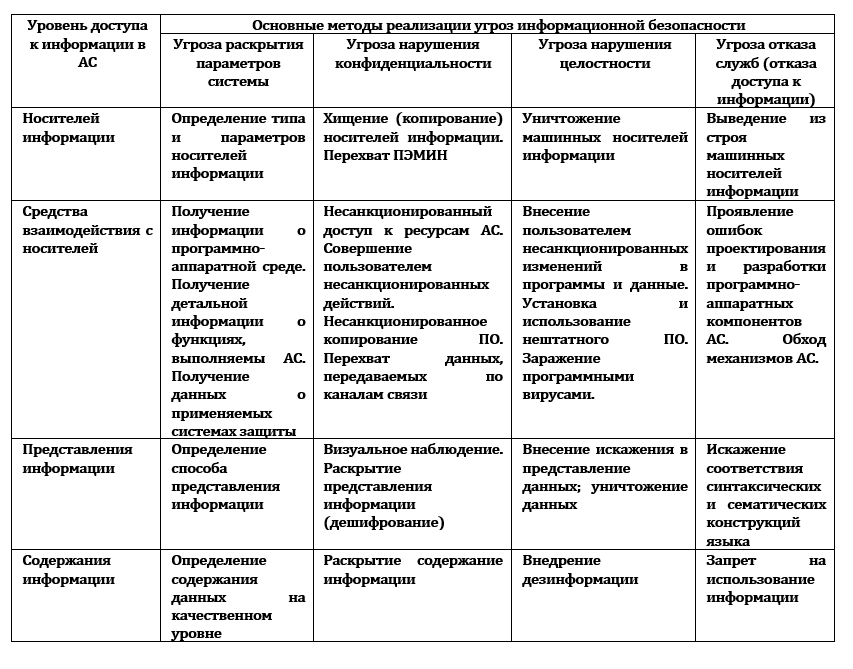
\includegraphics[width=1.2\linewidth]{screenshot002}
		\caption{}
		\label{fig:screenshot002}
	\end{figure}
	
	\textbf{Требования для работы с информации 1-го класса:}
	\begin{enumerate}
		\item Осведомление сотрудников о закрытости данной информации
		\item Общее ознакомление сотрудников с основными возможными методами атак на информацию
		\item Ограничение физического доступа
		\item Полный набор документации по правилам выполнения операций с данной информацией
	\end{enumerate}

	
	\textbf{Требования для работы с информацией 2-го класса:}
	\begin{enumerate}
		\item Расчёт рисков атак на информацию
		\item Поддержание списка лиц, имеющих доступ к данной информации
		\item По возможности выдача подробной информации под расписку (в т.ч. электронной)
		\item Автоматическая система проверки целостности системы и её средств безопасности
		\item Надёжные схемы физической транспортировки
		\item Обязательное шифрование при передаче по линиям связи
		\item Схема бесперебойного питания ЭВМ
	\end{enumerate}

	
	\textbf{Требования для работы с информацией 3-го класса:}
	\begin{enumerate}
		\item Детальный план спасения либо надёжного уничтожения информации в аварийных ситуациях (пожар, наводнение, взрыв)
		\item Защита ЭВМ либо носителей информации от повреждения водой и высокой температурой 
		\item Криптографическая проверка целостности информации
	\end{enumerate}

	
	\begin{figure}
		\centering
		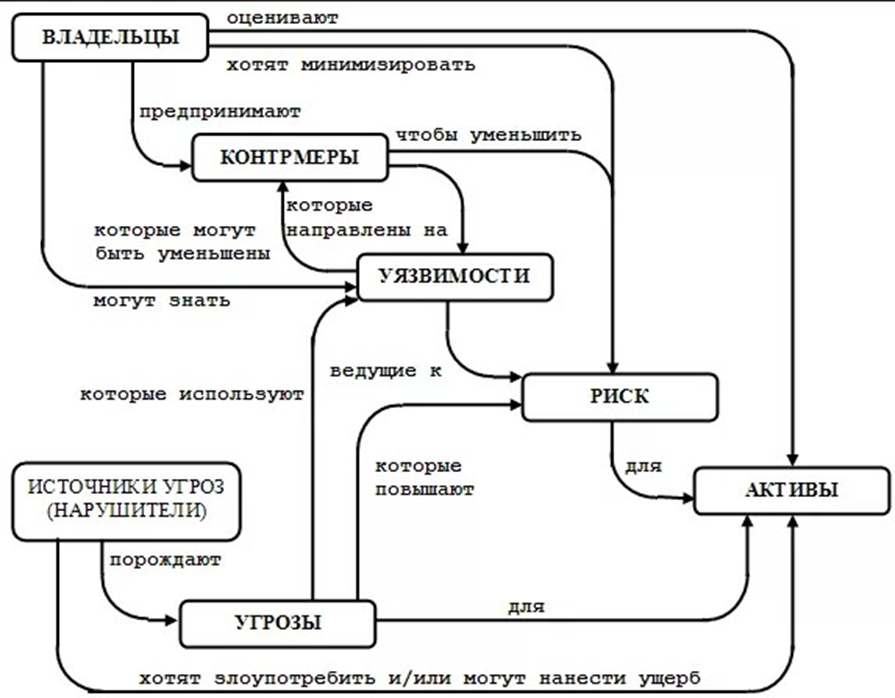
\includegraphics[width=1\linewidth]{screenshot001}
		\caption{}
		\label{fig:screenshot001}
	\end{figure}
	
	
	\section{Правовые и организационные методы защиты информациии в информационно вычислительных системах}
	\subsection{Стандарты и спецификации в области информационной безопасности}
	
	Вопросы
	\begin{enumerate}
		\item Стандарт ISO 15408 "Критерии оценки безопасности технологий"
		\item критерии оценки надёжных компьютерных систем
	\end{enumerate}
	\subsubsection{Стандарт ISO 15408 "Критерии оценки безопасности технологий"}
	
	Стандарт ISO 15408 принят 1 декабря 1999 часто называется Общие критерии (ОК)
	
	Характиристика угроз :
	\begin{enumerate}
		\item источник угроз
		\item методы воздействия
		\item уязвимыми местами которые могут быть использованы
		\item ресурсы которые могут пострадать
	\end{enumerate} 
	Уязвимые места возникают тогда
	\begin{enumerate}
		\item требования безопасности 
		\item проектирование 
		\item эксплуатация
	\end{enumerate}

	2 основные требования безопасности стандарт ISO 15408:
	\begin{enumerate}
		\item Функциональные, соотведстует активному аспекту зациты предьявляемой к функцим безопасности и реализующим их механизмам
		\item Требования доверия, СООТВЕДСТВУЮЩИЕ ПАССИВНОМУ АСПЕКТУ.
	\end{enumerate}
	% В общих свединиях введена иерархия класс=семейно-компонет-элемент
	Классы функциональных требований ОК:
	\begin{enumerate}
		\item Индификация и аутодификация
		\item защата данных пользователя
		\item приватность 
		\item использование ресурсов
		\item крипрографическая подержка
	\end{enumerate}
	
	Форма предоставления теребований доверия принцепи не чем не отличается от функциональным, отличие что кажждое действие пренаждлежит одному типу:
	\begin{enumerate}
		\item действия разработчиков
		\item предоставление и содержание свидетельства
		\item действия оценщиков
	\end{enumerate}

	Классы требований доверия безопасности ОК:
	\begin{enumerate}
		\item Разработка
		\item подержка ЖЦ
		\item тестирование
		\item оценка уязвимости
		\item поставка и эксплуатация
		\item упровление конфигурацией 
		\item руковонство
		\item поддержка доверия
		\item оценка профиля защиты
		\item оценка задания по безопасности
	\end{enumerate}

	В ОК введене оценочные уровни (7 штук):
	\begin{enumerate}
		\item Оценочный уровень доверия 1. Анализ функциональных спецификаций, специальных интерфейсов, а текже независемое тестирование. Урове нь применим, когда угрозы не рассматириваются как сериёзные
		\item Оценочный уровень доверия 2. Предусматривает наличие проекта верхнего уровня объекта оценки выборочное тестирование, анализ стойкости функции безопасности, поиск разработчиком явных уязвимых мест.
		\item Оценочный уровень доверия 3.Ведётся контроль среды разработки и упровления конфигурацией объектов оценки.
		\item Оценочный уровень доверия 4. Полная спецификация интерфейсов, проектов нижнего уровня, анализ подмножества реализации, применение неформальный модели политики безопасности, независимый анализ уязвимых мест, автоматизация управления конфигурацией. 
		\item Оценочный уровень доверия 5. в дополнение к предудущим предусматривает применение формальцной модели политика политики безопасности полуформальных функциональноной спецификации и проекта. Необходимо проведение анализа скрытых каналов разработчиками и оценщиками. 
		\item Оценочный уровень доверия 6. Реализация должна быть представленна в структурном види. Анализ соотведствия распостраняется на проект нижнего уровня
		\item Оценочный уровень доверия 7. Предусматривает формальныую вирификацию проекта обхекта оценки. Он применим к ситуациям черезвычайно высогого риска.
	\end{enumerate}
	\subsubsection{Критерии оценки надёжных компьютерных систем}
	Степень доверия или надежность систем, оценивается по двум основным критериям 
	\begin{enumerate}
		\item Политика безопасности - набор законов, правил норм поведения, определяющих, как организация обрабатывает, защищает и распостраняет информцию.
		\item Гарантированость --- мера доверия, которая может быть оказана архетектуре и реализации системы. Гарантированность может происходить как из тестирования, так и из проверки общего замысла и исполннение системы в целом и её компонентов.
		\item Надажнось вычислительная база --- это совокупность защатных механизмов компьютерной системы, отвечающих за проведение в жизни политики безопасности
		\item Основное назначение надежной вычислительной базы --- выполнит финкции монитора обращений, то есть контролировать доступность выполнения субъектами определеных операций нал объектами.
	\end{enumerate}
	От монитора обращение требуется выполнение трех свойств:
	\begin{enumerate}
		\item Изолированость. Монитор должен быть защащен от отслуживания свией работы.
		\item Полнота. Монитор должен вызывать при каждом обращении не должно быть спрособов его обхода
		\item Верифицируемость. Монитор должен быть компактным, чтобы его можно было проанализировать и протестировать, будучи уверенным в полноте тестировании.
	\end{enumerate}
	Основыне элементы политики безоасности 
	\begin{enumerate}
		\item произволоное упровление доступом
		\item безопасность повторного использование объектов
		\item метки безопасности
		\item принудительное упровление доступом
	\end{enumerate}


	\section{Методы идентификации и аутентификации}
	\subsection{Идентификация и аутентификация}
	
	\subsubsection{Требования к идентификации и аутентификации}
	С каждым зарегистрированным в компьютерной системе субъектом (пользователем или процессом, действующим от имени пользователя) связана некоторая информация, однозначно идентифицирующая его. Это может быть число или строка символов, именующие данный субъект. Такую информацию называют идентификатором субъекта. Имея идентификатор, зарегистрированный в сети пользователь считается легальным (заданным); остальные субъекты относятся к нелегальным.
	
	Прежде чем получить доступ к ресурсам компьютерной системы, пользователь должен пройти процесс первичного взаимодействия с компьютерной системой, который включает две стадии идентификацию и аутентификацию.
	
	Идентификация — это процедура распознавания пользователя по его идентификатору (имени). Эта функция выполняется в первую очередь, когда пользователь делает попытку войти в сеть. Он сообщает системе по ее запросу свой идентификатор, и система проверяет в своей базе данных его наличие.
	
	Аутентификация — процедура проверки подлинности, позволяющая достоверно убедиться, что пользователь является именно тем, кем он себя объявляет. При проведении аутентификации проверяющая сторона убеждается в подлинности проверяемой стороны; при этом проверяемая сторона тоже активно участвует в процессе обмена информацией. Обычно пользователь подтверждает свою идентификацию, вводя в систему уникальную, не известную другим пользователям информацию о себе (например, пароль или сертификат).
	
	Идентификация и аутентификация — взаимосвязанные процессы распознавания и проверки подлинности субъектов (пользователей). Именно от них зависит решение системы, можно ли разрешить доступ к ресурсам системы конкретному пользователю или процессу. 
	\subsubsection{Авторизация с точки зрения количества и вида зарегистрированных пользователей}
	Авторизация – предоставление прав (или привилегий), позволяющих владельцу иметь законный доступ к системе или к её объектам. Механизм авторизации часто называют подсистемой управления доступом, которая также требует проектирования. Процесс авторизации включает в себя идентификацию и аутентификацию пользователей.
	
	В системе зарегистрирован один пользователь
	
	Данный пользователь является и прикладным пользователем, и администратором безопасности. Здесь источником потенциальной угрозы является только сторонний сотрудник предприятия, а вся задача защиты сводится к контролю доступа в компьютер (либо в систему), т.е. к парольной защите.
	
	Данный случай является вырожденным и нами далее не рассматривается, т.к. в соответствии с формализованными требованиями к защите информации от НСД даже при защите конфиденциальной информации предполагается обязательное наличие администратора безопасности.
	
	В системе зарегистрированы администратор безопасности и один прикладной пользователь
	
	Общий случай функционирования системы с одним прикладным пользователем – это наличие в системе администратора безопасности и только одного прикладного пользователя. В задачи администратора безопасности здесь входит ограничение прав прикладного пользователя по доступу к системным (администратора безопасности) и иным ресурсам компьютера. В частности, может ограничиваться набор задач, разрешенных для решения на компьютере, набор устройств, которые могут быть подключены к компьютеру (например, внешний модем, принтер и т.д.), способ сохранения обрабатываемых данных (например, на дискетах только в шифрованном виде) и т.д.
	
	В данном случае потенциальным злоумышленником в части несанкционированного использования ресурсов защищаемого объекта может являться как сторонний сотрудник предприятия, так и собственно прикладной пользователь. Заметим, что прикладной пользователь здесь может выступать в роли сознательного нарушителя, либо стать «инструментом» в роли стороннего нарушителя, например, запустив по чьей-либо просьбе какую-нибудь программу).
	
	В системе зарегистрированы администратор безопасности и несколько прикладных пользователей
	
	Кроме администратора безопасности, в системе может быть заведено несколько прикладных пользователей. При этом ресурсами защищаемого компьютера могут пользоваться несколько сотрудников, решая различные задачи. Ввиду этого информационные и иные ресурсы защищаемого объекта должны между ними разграничиваться.
	
	В данном случае к потенциальным нарушителям добавляется санкционированный прикладной пользователь, целью которого может служить НСД к информации, хранимой на защищаемом объекте другим пользователем.
	
	При использовании компьютера (прежде всего, рабочей станции) в составе ЛВС, помимо локальных ресурсов защищаемого объекта, защите подлежат сетевые ресурсы.
	
	В этом случае между пользователями могут разграничиваться права по доступу к серверам, сетевым службам, разделенным сетевым ресурсам (общим папкам и устройствам, например, к сетевым принтерам) и т.д.
	
	Здесь злоумышленник (санкционированный пользователь) может осуществлять попытку получить НСД к сетевому ресурсу, к которому ему доступ не разрешен, с целью осуществления на него атаки с рабочей станции. 
	\subsubsection{Классификация задач идентификации и аутентификации}
	Цель идентификации – установить тождественность или подлинность объекта (товара) его основополагающим характеристикам.
	
	На современном этапе задачами идентификации являются:
	
	- определение структуры, норм и правил в области идентификации товаров;
	
	- разработка основополагающих критериев, пригодных для целей идентификации однородных групп, конкретных видов и наименований товаров;
	
	- исследование потребительских свойств товаров и показателей, их характеризующих, для выявления наиболее достоверных критериев идентификации;
	
	- совершенствование стандартов, ТУ и другой нормативной документации путем включения в нее показателей качества для целей идентификации;
	
	- совершенствование методов идентификации товаров, и в первую очередь экспресс-методов, позволяющих с достаточно высокой степенью достоверности определять все основополагающие характеристики товаров, особенно товароведные.
	
	Объектами идентификации являются продукция, услуги, ценные бумаги (деньги, акции, векселя и др.), информация, рабочая сила и другие объекты коммерческой деятельности. В данном учебном пособии разберем лишь одну группу объектов – продукцию, которая вовлекается в процесс купли-продажи и становится товаром. Именно об идентификации продовольственных товаров в сфере торговли и у потребителя, приобретающего товары, пойдет речь, хотя следует отметить, многие рассматриваемые вопросы в равной степени могут быть отнесены и к непродовольственным товарам.
	
	Субъектами, осуществляющими идентификацию товаров, являются все участники рыночных отношений: изготовитель – на стадии приемки сырья, полуфабрикатов, комплектующих изделий и при отпуске готовой продукции;
	
	продавец – на стадиях заключения договоров купли-продажи, приемки товаров и подготовки их к продаже. Потребитель также проводит идентификацию приобретаемого товара, делая это чаще всего неосознанно и не имея достаточной квалификации, ориентируясь лишь на собственный житейский опыт и знания.
	
	Классификации механизмов авторизации, реализованных в системах защиты:
	
	- классификация по функциональному назначению(контроль загрузки, контроль функционирования);
	
	- классификация по принадлежности идентификаторов и паролей(пользователь, ответственное лицо);
	
	- классификация по субъекту их задания(администратор, пользователь, ответственное лицо) ;
	
	- классификация по способу ввода идентификатора и пароля(ввод с клавиатуры, ввод с внешнего устройства);
	
	- классификация по способу хранения идентификатора и пароля (локально на защищаемом объекте, удаленно на сервере). 
	\subsubsection{Методы идентификации и установления подлинности субъектов и различных объектов}
	Объект идентификации и установление подлинности.
	
	Идентификация- это присвоение какому-либо объекту или субъекту уникального образа, имени или числа. Установление подлинности (аутентификация) заключается в проверке, является ли проверяемый объект (субъект) в самом деле тем за кого себя выдает.
	
	Объектами идентификации могут быть:
	
	- человек (оператор, пользователь, оператор);
	
	- техническое средство (терминал, дисплей, компьютер и т.д.);
	
	- документы (распечатки, листинги и т.п.);
	
	- носители информации (магнитные диски, ленты и т.п.);
	
	- информация (табло, информация на дисплее).
	
	Идентификация может быть произведена как специальным персоналом, так и техническими средствами.
	
	Идентификация и установление подлинности личности. В качестве признака подлинности личности внешние признаки (рост, вес, формы отдельных частей тела и т.п.) правда со временем параметры человека меняются, но с развитием техники растет и точность прогнозирования этих изменений (отпечатки пальцев, голос и т.д.). Кроме антропологических параметров более внимательно необходимо относится к конфиденциальности, так как записанная информация на носителях является ключом к информации, подлежащей защите. Для этого существует система аутентификации “ключ-замок”. Система “ключ-замок” имеет локальный применение. Одним из распространенным методом аутентификации является присвоение лицу или объекту уникального имени или числа - пароля и хранение его в компьютерной системе. При входе в компьютерную систему пользователь открывает доступ к разрешенной только ему информации. 
	Алгоритм идентификации компьютерной системы представлен (Рисунок . 3). Наиболее высокий уровень входа в систему разделение кода на две части: одну запоминаемую пользователем и вводимую вручную, вторую с помощью магнитной или иной карточкой.
	
	На случай защиты запоминаемой части пароля от получения ее нарушителем путем физического принуждения пользователя, возможно, будет полезно в вычислительной системе предусмотреть механизм тревожной сигнализации, основанной на применении ложного пароля. Ложный пароль запоминается пользователем одновременно с действительным и сообщается преступнику в экстренной ситуации.
	
	Однако, учитывая опасность для жизни пользователя необходимо в компьютерной системе одновременно со скрытой сигнализацией предусмотреть механизм обязательного выполнения требований преступника, воспользовавшись средствами аутентификации законного пользователя.
	
	Идентификация и установление подлинности технических средств. При организации системы защиты информационных процессов является идентификация подлинности технических средств. Данный уровень защиты осуществляется с помощью паролей. Пароль используется не только для пользователя и терминала по отношению к системе, но и для обратного установления подлинности компьютера по отношению к пользователю. Это используется для работы с удаленным объектом. В этом случае используются одноразовые пароли или более сложные системы шифрования информации. 
	\begin{figure}
		\centering
		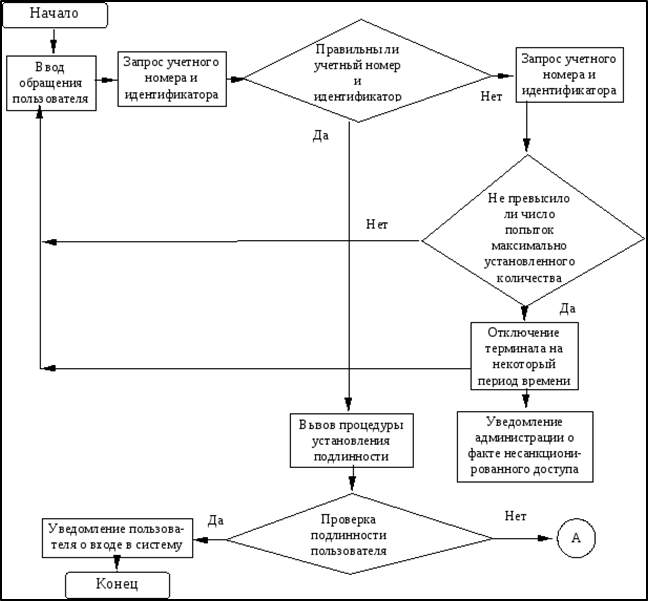
\includegraphics[width=0.7\linewidth]{screenshot003}
		\caption{}
		\label{fig:screenshot003}
	\end{figure}
	
	Идентификация и установление подлинности документов. 
	В компьютерных системах документами являются распечатки, листинги, перфоленты, перфокарты, магнитные носители и т.д. Для этого случая используется два подхода:
	 получение документа, сформированного непосредственно в КС и на ее документирования;
	 получение ее с удаленных объектов КС.
	В первом случае подлинность гарантируется системой, имеющие средства защиты от НСД, а также физическими характеристиками печатающего устройства, присущие только этой системы. При недостаточности необходимо использовать криптографическое преобразование. Это особенно актуально для второго случая, когда документ доставляется через неохраняемую территорию с территории удаленного объекта. При этом к носителю прилагаются документы с подписями ответственных лиц, заверенными печатями.
	При неавтоматизированном обмене информацией подлинность документов удостоверяется личной подписью человека, автора документа. Проверка осуществляется визуально по личным документам.
	При автоматизированной передаче документов по каналам связи, расположенным на неконтролируемой территории, меняются условия обмена. Так как в этом случае подделка подписи документов является относительно простой, то используется так называемая электронная подпись. Этим пользуются организации занимающими банковскими и другими жизненно важной деятельностью. При этом участники нуждаются в защите от преднамеренных НСД в виде:
	 отказа отправителя от переданного сообщения;
	 изменения получателем полученного сообщения;
	 маскировки отправителя под другого сообщения.
	Обеспечение защиты каждой стороны, участвующей в обмене информации, осуществляется с помощью ведения специальных протоколов. Для верификации используют следующие положения:
	 отправитель вносит в передаваемую информацию свою электронную подпись, представляющую собой дополнительную информацию, зависящую от передаваемых данных, имени получателя и некоторой закрытой информации, который обладает только отправитель;
	 получатель должен иметь возможность удостовериться в том, что в составе сообщения подпись есть подлинная подпись отправителя;
	 получение правильной подписи отправителя возможно только при использовании закрытой информации, которой обладает только отправитель;
	 для исключения возможности повторного использования устаревшего сообщения верификация должна зависеть от времени.
	Подпись сообщения представляет собой способ шифрования сообщения с помощью криптографического преобразования. Закрываемым элементом в преобразовании является код ключа.
	Идентификация и установление подлинности информации на средствах ее отображения и печати. В компьютерных системах с централизованной обработкой данных и относительно низкими требованиями к защите установлении ее подлинности на технических средствах отображения информации гарантируется данной КС. Однако с усложнением системы увеличивается и вероятность возникновения НСД к информации, ее модификации и хищению. Поэтому в более ответственных случаях отдельные сообщения или блоки информации подвергаются специальной защите, которая заключается в создании средств повышения достоверности информации, ее криптографического преобразования. Установление подлинности полученной информации, включая отображение на табло и терминалах, заключается в контроле обеспечения достоверности информации, результатов дешифрования полученной информации до отображения ее на дисплее. Подлинность информации на средствах ее отображения тесно связана с подлинностью документов. Поэтому все положения приведены ранее справедливы и для этого случая. Чем ближе к полю отображения (бумажному носителю) эта процедура приближается, тем достовернее отображаемая информация.
	
	\subsubsection{Биометрическая аутентификация пользователей}
	Привычные системы аутентификации на сегодня не всегда удовлетворяют требованием политики информационной безопасности предприятия или компании. Все большую популярность набирает биометрическая аутентификация пользователя, разрешающая аутентифицировать пользователя с помощью считывания его физиологических данных.
	Методы аутентификация основывающийся на паролях имеют недостаток: многоразовый пароль можно скомпрометировать разными способами. USB-токкены и смарт-карты можно потерять, скопировать. Биометрические методы аутентификации не имеют эти недостатки. К основным плюсам таких методов относят:
	 большой уровень достоверности аутентификации по биометрическим параметрам из-за их уникальности
	 неотделимость биометрических параметров от пользователя;
	 сложность фальсификации биометрических признаков.
	В качестве биопараметров используют следующие:
	 форма кисти руки;
	 отпечаток пальца;
	 размер и форма лица;
	 узор сетчатки глаза и радужной оболочки;
	 особенности голоса.
	Схема работы биометрической системы аутентификации
	При процессе регистрации в системе пользователь должен показать один или несколько раз биометрический признак, по которому происходит дальнейшая аутентификация. Эти признаки в системе регистрируются как контрольный образец пользователя. Этот образец обрабатывается системой для получения ЭИП (эталонный идентификатор пользователя). ЭИП – числовая последовательность, из которой нельзя восстановить первоначальный образец. При прохождении аутентификации пользователем, сравнивается эталонные ЭИП и ЭИП при прохождении аутентификации. Поскольку эти 2 параметра никогда не совпадут, существует параметр отвечающий за степень совпадения. На основе этой степени совпадения система решает о прохождении аутентификации.
	Ошибочный отказ (FRR)- это отказ, когда система не подтверждает законного пользователя. Такие отказы бывают 1 на 100.
	Ошибочное подтверждение (FAR) — подтверждение, когда система подтверждает аутентификацию незаконного пользователя. ТАкие ошибки бывают 1 на 10000.
	Дактилоскопическая система аутентификации
	Одна из причин широкого использования таких систем, это наличие громадных банков данных по отпечаткам пальцев. Основные пользователи таких систем являются сотрудники гос. служб или банковские компании. Основные компоненты дактилоскопической системы аутентификации:
	 сканер
	 ПО идентификации
	 ПО аутентификации
	
\end{document}